% Options for packages loaded elsewhere
\PassOptionsToPackage{unicode}{hyperref}
\PassOptionsToPackage{hyphens}{url}
%
\documentclass[
]{article}
\usepackage{amsmath,amssymb}
\usepackage{iftex}
\ifPDFTeX
  \usepackage[T1]{fontenc}
  \usepackage[utf8]{inputenc}
  \usepackage{textcomp} % provide euro and other symbols
\else % if luatex or xetex
  \usepackage{unicode-math} % this also loads fontspec
  \defaultfontfeatures{Scale=MatchLowercase}
  \defaultfontfeatures[\rmfamily]{Ligatures=TeX,Scale=1}
\fi
\usepackage{lmodern}
\ifPDFTeX\else
  % xetex/luatex font selection
\fi
% Use upquote if available, for straight quotes in verbatim environments
\IfFileExists{upquote.sty}{\usepackage{upquote}}{}
\IfFileExists{microtype.sty}{% use microtype if available
  \usepackage[]{microtype}
  \UseMicrotypeSet[protrusion]{basicmath} % disable protrusion for tt fonts
}{}
\makeatletter
\@ifundefined{KOMAClassName}{% if non-KOMA class
  \IfFileExists{parskip.sty}{%
    \usepackage{parskip}
  }{% else
    \setlength{\parindent}{0pt}
    \setlength{\parskip}{6pt plus 2pt minus 1pt}}
}{% if KOMA class
  \KOMAoptions{parskip=half}}
\makeatother
\usepackage{xcolor}
\usepackage[margin=1in]{geometry}
\usepackage{graphicx}
\makeatletter
\def\maxwidth{\ifdim\Gin@nat@width>\linewidth\linewidth\else\Gin@nat@width\fi}
\def\maxheight{\ifdim\Gin@nat@height>\textheight\textheight\else\Gin@nat@height\fi}
\makeatother
% Scale images if necessary, so that they will not overflow the page
% margins by default, and it is still possible to overwrite the defaults
% using explicit options in \includegraphics[width, height, ...]{}
\setkeys{Gin}{width=\maxwidth,height=\maxheight,keepaspectratio}
% Set default figure placement to htbp
\makeatletter
\def\fps@figure{htbp}
\makeatother
\setlength{\emergencystretch}{3em} % prevent overfull lines
\providecommand{\tightlist}{%
  \setlength{\itemsep}{0pt}\setlength{\parskip}{0pt}}
\setcounter{secnumdepth}{-\maxdimen} % remove section numbering
\ifLuaTeX
  \usepackage{selnolig}  % disable illegal ligatures
\fi
\IfFileExists{bookmark.sty}{\usepackage{bookmark}}{\usepackage{hyperref}}
\IfFileExists{xurl.sty}{\usepackage{xurl}}{} % add URL line breaks if available
\urlstyle{same}
\hypersetup{
  pdftitle={311306435},
  hidelinks,
  pdfcreator={LaTeX via pandoc}}

\title{311306435}
\author{}
\date{\vspace{-2.5em}2023-07-18}

\begin{document}
\maketitle

\begin{verbatim}
## package 'DirichletReg' successfully unpacked and MD5 sums checked
## 
## The downloaded binary packages are in
##  C:\Users\Yuval-PC\AppData\Local\Temp\RtmpikcL46\downloaded_packages
\end{verbatim}

\begin{verbatim}
## package 'scatterplot3d' successfully unpacked and MD5 sums checked
## 
## The downloaded binary packages are in
##  C:\Users\Yuval-PC\AppData\Local\Temp\RtmpikcL46\downloaded_packages
\end{verbatim}

\begin{verbatim}
## package 'MASS' successfully unpacked and MD5 sums checked
## 
## The downloaded binary packages are in
##  C:\Users\Yuval-PC\AppData\Local\Temp\RtmpikcL46\downloaded_packages
\end{verbatim}

\begin{verbatim}
## package 'MCMCprecision' successfully unpacked and MD5 sums checked
## 
## The downloaded binary packages are in
##  C:\Users\Yuval-PC\AppData\Local\Temp\RtmpikcL46\downloaded_packages
\end{verbatim}

\begin{verbatim}
## package 'ggpubr' successfully unpacked and MD5 sums checked
## 
## The downloaded binary packages are in
##  C:\Users\Yuval-PC\AppData\Local\Temp\RtmpikcL46\downloaded_packages
\end{verbatim}

Question 1

Question 2

Question 3
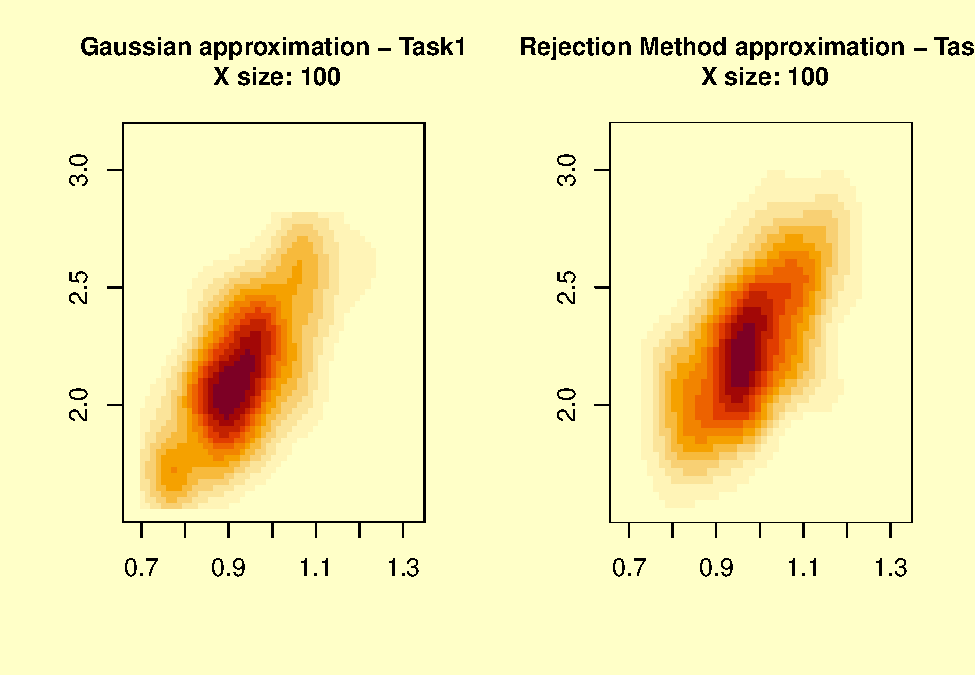
\includegraphics{take_home_q1_q2_q3_files/figure-latex/unnamed-chunk-2-1.pdf}
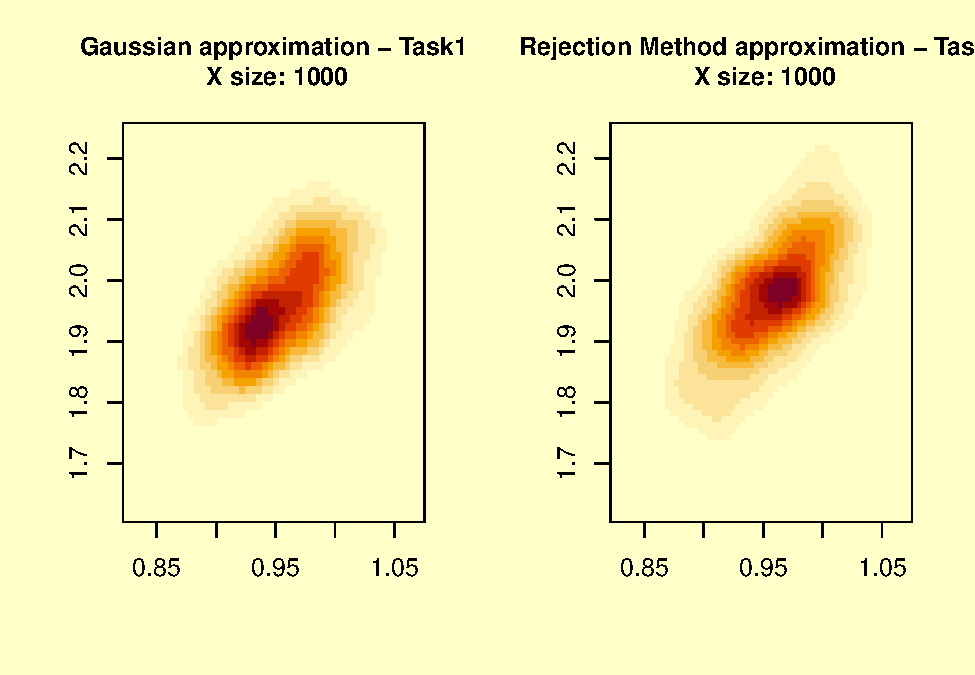
\includegraphics{take_home_q1_q2_q3_files/figure-latex/unnamed-chunk-2-2.pdf}
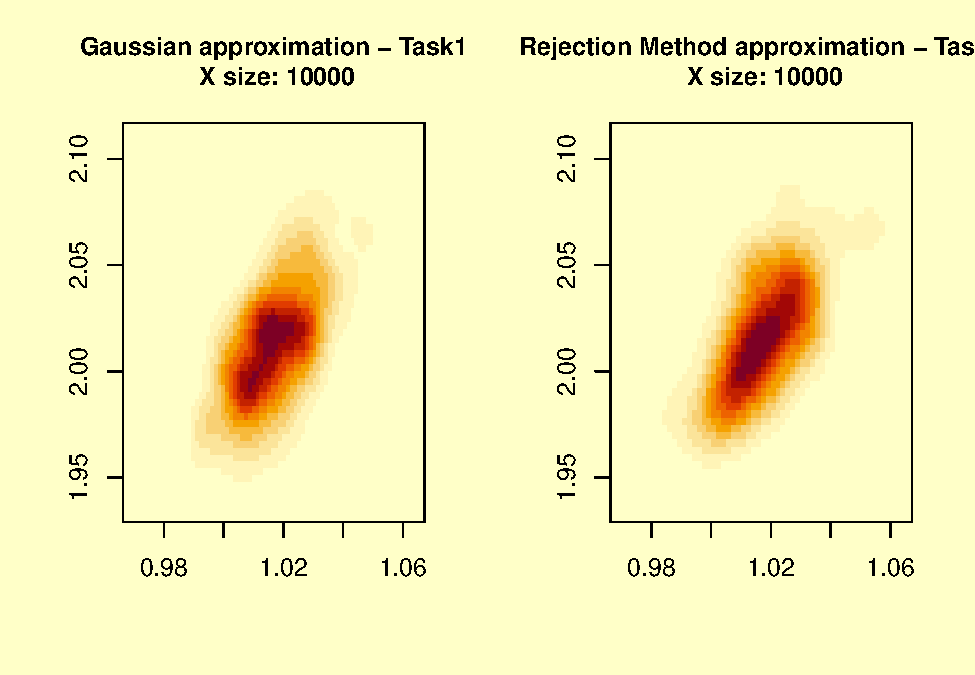
\includegraphics{take_home_q1_q2_q3_files/figure-latex/unnamed-chunk-2-3.pdf}

\begin{verbatim}
## package 'plyr' successfully unpacked and MD5 sums checked
## 
## The downloaded binary packages are in
##  C:\Users\Yuval-PC\AppData\Local\Temp\RtmpikcL46\downloaded_packages
\end{verbatim}

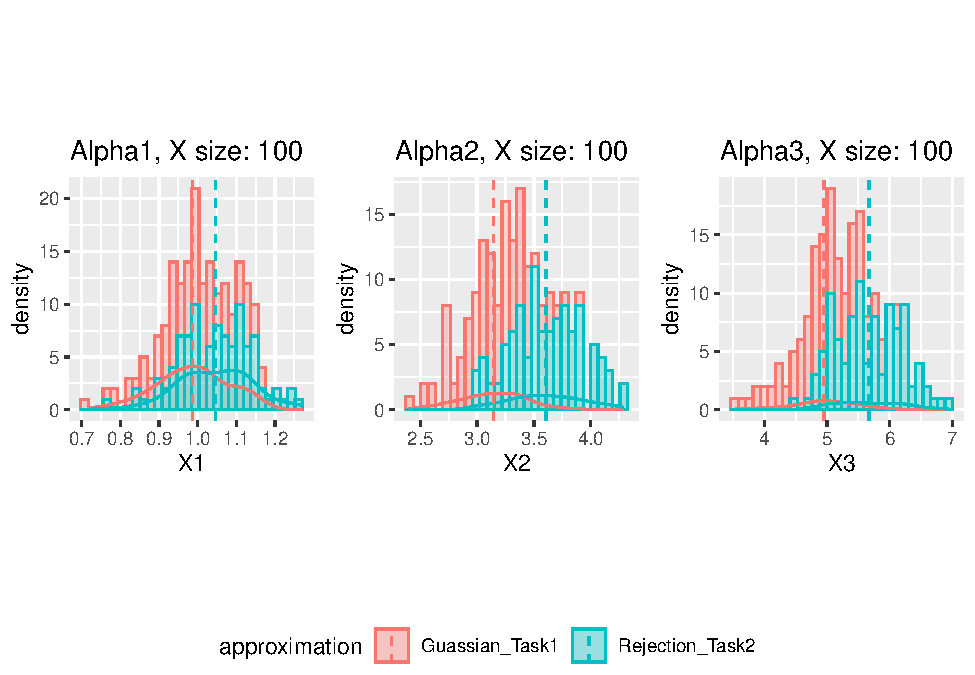
\includegraphics{take_home_q1_q2_q3_files/figure-latex/unnamed-chunk-3-1.pdf}
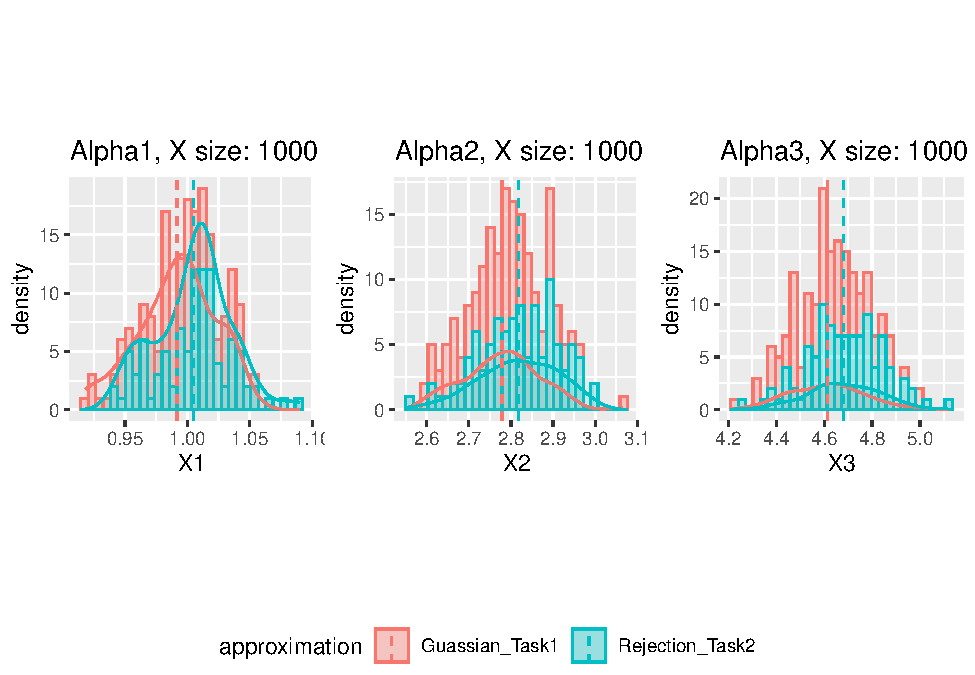
\includegraphics{take_home_q1_q2_q3_files/figure-latex/unnamed-chunk-3-2.pdf}
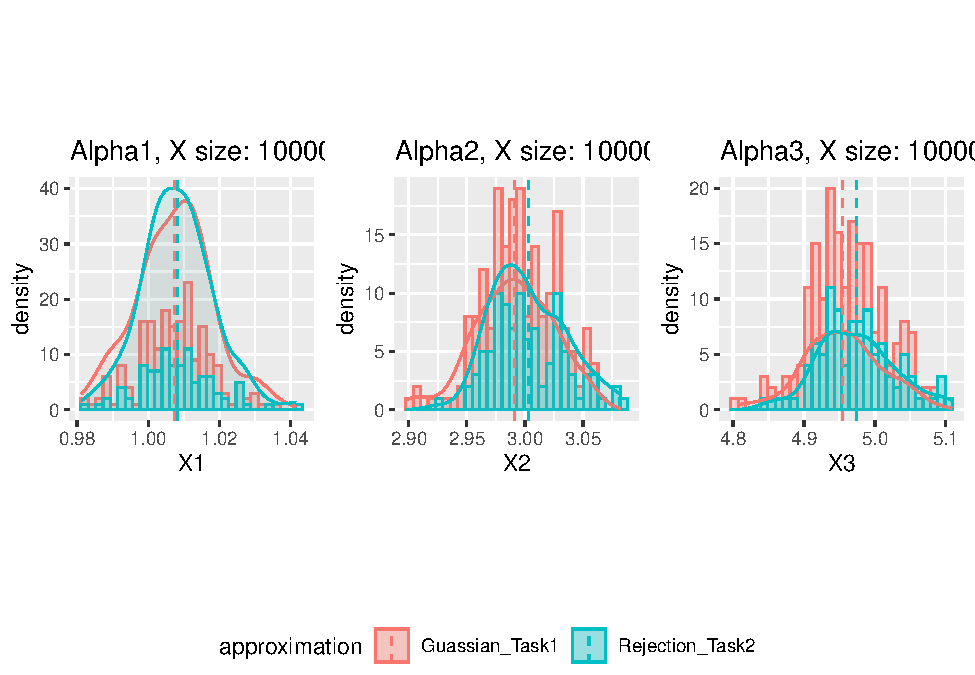
\includegraphics{take_home_q1_q2_q3_files/figure-latex/unnamed-chunk-3-3.pdf}

\begin{verbatim}
## [1] 2
## [1] "x_size 64"
## [1] "x_size 128"
## [1] "x_size 256"
## [1] "x_size 512"
## [1] "x_size 1024"
## [1] "x_size 2048"
## [1] "x_size 4096"
## [1] "x_size 8192"
## [1] "x_size 16384"
## [1] "x_size 32768"
## [1] "x_size 65536"
## [1] 3
## [1] "x_size 64"
## [1] "x_size 128"
## [1] "x_size 256"
## [1] "x_size 512"
## [1] "x_size 1024"
## [1] "x_size 2048"
## [1] "x_size 4096"
## [1] "x_size 8192"
## [1] "x_size 16384"
## [1] "x_size 32768"
## [1] "x_size 65536"
## [1] 4
## [1] "x_size 64"
## [1] "x_size 128"
## [1] "x_size 256"
## [1] "x_size 512"
## [1] "x_size 1024"
## [1] "x_size 2048"
## [1] "x_size 4096"
## [1] "x_size 8192"
## [1] "x_size 16384"
## [1] "x_size 32768"
## [1] "x_size 65536"
## [1] 5
## [1] "x_size 64"
## [1] "x_size 128"
## [1] "x_size 256"
## [1] "x_size 512"
## [1] "x_size 1024"
## [1] "x_size 2048"
## [1] "x_size 4096"
## [1] "x_size 8192"
## [1] "x_size 16384"
## [1] "x_size 32768"
## [1] "x_size 65536"
\end{verbatim}

\includegraphics{take_home_q1_q2_q3_files/figure-latex/unnamed-chunk-4-1.pdf}
Question 4

\begin{verbatim}
## Q3_non_zeros
##  1  2  3 
## 50 38 12
\end{verbatim}

\begin{verbatim}
## Q4_non_zeros
##  1  2  3  4 
## 53 31 13  3
\end{verbatim}

\includegraphics{take_home_q1_q2_q3_files/figure-latex/count non zero-1.pdf}
We can see that in both cases the samples are affected by one component
of the distribution, although there are 3 or 4 components. Its look like
adding the fourth component did not improved the explainability of the
data that much.
\includegraphics{take_home_q1_q2_q3_files/figure-latex/finds similar groups-1.pdf}
The goal of that plot is to check what is the best k for k-means
algorithm. By the elbow method, its look like it is best to select k=3
for Q3 and k=4 for Q4. By choosing k=8 to k=10 the loss is almost 0.

\begin{verbatim}
## package 'ggtern' successfully unpacked and MD5 sums checked
## 
## The downloaded binary packages are in
##  C:\Users\Yuval-PC\AppData\Local\Temp\RtmpikcL46\downloaded_packages
\end{verbatim}

\includegraphics{take_home_q1_q2_q3_files/figure-latex/unnamed-chunk-5-1.pdf}
\includegraphics{take_home_q1_q2_q3_files/figure-latex/unnamed-chunk-5-2.pdf}
By looking at the trinary graph, its look like there are few different
groups with different behaviors and distributions. Although the elbow
method suggets to take for k-means k=3, I think it is much more suitable
to take k=10. In that way, groups with no contribution in one of the
components will attributed to separate cluster than those of affected
from all the components like the points in the middle of the triangle.
Yet, using k-means is not optimal as the centers are spatial and they
separate gorups that suppose to be together like the ones in the left
upper edge.

\begin{verbatim}
## package 'fpc' successfully unpacked and MD5 sums checked
## 
## The downloaded binary packages are in
##  C:\Users\Yuval-PC\AppData\Local\Temp\RtmpikcL46\downloaded_packages
\end{verbatim}

\begin{verbatim}
## package 'dbscan' successfully unpacked and MD5 sums checked
## 
## The downloaded binary packages are in
##  C:\Users\Yuval-PC\AppData\Local\Temp\RtmpikcL46\downloaded_packages
\end{verbatim}

\includegraphics{take_home_q1_q2_q3_files/figure-latex/unnamed-chunk-6-1.pdf}
In this section we try to use DBSCAN in order to find better clusters.
The assumption of DBSCAN is that clusters are densed in the space more
than other areas in the space. It groups densely grouped data points
into single cluster. It performs better on separating the edges to other
groups than the points that affected from 2-3 components.

\begin{verbatim}
## package 'kernlab' successfully unpacked and MD5 sums checked
## 
## The downloaded binary packages are in
##  C:\Users\Yuval-PC\AppData\Local\Temp\RtmpikcL46\downloaded_packages
\end{verbatim}

\includegraphics{take_home_q1_q2_q3_files/figure-latex/spectral clustering-1.pdf}
In this section we apply spectral clustering with splinedot kernel. The
goal was to find a kernel that separates the best between the zero
components group to the the groups that are contributed from all the
components. There are real 5 groups (and 3 more groups that catched
single dots). This is the best clusters we got up to this point.

\includegraphics{take_home_q1_q2_q3_files/figure-latex/unnamed-chunk-7-1.pdf}

\includegraphics{take_home_q1_q2_q3_files/figure-latex/unnamed-chunk-8-1.pdf}
By examine the cluster, we can find 3 kinds of clusters: 1. One
component cluster - affected by one component only (Alpha3 = 0.99998 for
example) 2. Two components cluster. We can see that it is approximately
Guassian by looking at the heatmap 3. Three components cluster. We can
see that it is approximately Guassian by looking at the 3DScatterplot

To sum up we had Cluster 5, 8 - one component Clusters 1, 2, 4, 7(small)
- two components, approximately Guassian distributed cluster 3 - three
components, approximately Guassian distributed

So we can say that Q3 composed from 5 major groups, each from specific
as mentioned above.

\begin{verbatim}
## package 'GGally' successfully unpacked and MD5 sums checked
## 
## The downloaded binary packages are in
##  C:\Users\Yuval-PC\AppData\Local\Temp\RtmpikcL46\downloaded_packages
\end{verbatim}

\includegraphics{take_home_q1_q2_q3_files/figure-latex/unnamed-chunk-9-1.pdf}

\begin{verbatim}
## Error in download.file(url, destfile, method, mode = "wb", ...) : 
##   cannot open URL 'http://cran.us.r-project.org/bin/windows/contrib/4.3/klaR_1.7-2.zip'
\end{verbatim}

\begin{verbatim}
## package 'haven' successfully unpacked and MD5 sums checked
## 
## The downloaded binary packages are in
##  C:\Users\Yuval-PC\AppData\Local\Temp\RtmpikcL46\downloaded_packages
\end{verbatim}

\begin{verbatim}
## [1] 0
\end{verbatim}

\begin{verbatim}
## [1] 30
\end{verbatim}

\begin{verbatim}
## [1] 60
\end{verbatim}

\begin{verbatim}
## [1] 90
\end{verbatim}

\begin{verbatim}
## [1] 120
\end{verbatim}

\begin{verbatim}
## [1] 150
\end{verbatim}

\includegraphics{take_home_q1_q2_q3_files/figure-latex/unnamed-chunk-10-1.pdf}

\includegraphics{take_home_q1_q2_q3_files/figure-latex/unnamed-chunk-11-1.pdf}

\includegraphics{take_home_q1_q2_q3_files/figure-latex/unnamed-chunk-12-1.pdf}

Like in Q3, we separate to 3 kind of groups one component - 8(V3) 7(V1)
9(V2) 10(V4) two components - 1, 2, 3, 5, 6 three components - 4

I contrast to the case of Q3 with 3 dimensions, here the clustering
algorithms found it hard to separate the points into groups of 2
dimension and most of them spread over 3 dimensions. It is safe to say
that the samples are taken from a mixture of distributions, but here it
is harder to say what are the hidden distributions.

\end{document}
